%Example of use of oxmathproblems latex class for problem sheets
\documentclass{oxmathproblems}

%(un)comment this line to enable/disable output of any solutions in the file
%\printanswers

%define the page header/title info
\course{Algorithm Design and Analysis (Fall 2023)}
\sheettitle{Assignment 3\\Deadline: Dec 12, 2023} %can leave out if no title per sheet

\begin{document}
\begin{questions}

\miquestion[25]
Given a constant $k\in\mathbb{Z}^+$, we say that a vertex $u$ in an undirected graph \emph{covers} a vertex $v$ if the distance between $u$ and $v$ is at most $k$. In particular, a vertex $u$ covers all those vertices that are within distance $k$ from $u$, including $u$ itself. Given an undirected \emph{tree} $G=(V,E)$ and the parameter $k$, consider the problem of finding a minimum-size subset of vertices that covers all the vertices in $G$.
Design a polynomial time algorithm for this problem. Prove the correctness of your algorithm and analyze its running time.
You will receive 15 points if you can solve the problem for $k=1$.

\begin{Solution}

\textbf{First, consider the problem for $k=1$.} The algorithm for $k=1$ is below.

\begin{algorithm}[H]
    \caption{Cover all vertices with a minimum-size subset with $k=1$}
    \label{}
    \begin{algorithmic}[1]
        \State Boolean vectors \textit{covered}[ ] and \textit{marked}[ ] are initialized to \textit{False}.
        \State $subset=$[ ]
        \Comment{Record the resultant vertex found by algorithm.}
        \State Apply BFS on the tree $G$ and obtain an array $a[1,...,n]$ which sorts all vertices by their depths incrementally, and an array $pre[1,...,n]$ recording their parent vertex.
        \For{$i=n$ \textbf{to} $1$}
        \State \textbf{if} $covered[i]=True$\textbf{: continue}
            \State $u=pre[i]$
            \State $marked[u]=True$, $covered[u]=True$, $subset$.append($u$)
            \For{$v$ in $N(u)$} \Comment{$N(u)$ denotes children vertices of $u$}
                \State $covered[v]=True$
            \EndFor
        \EndFor
        \State \textbf{return} $subset$
    \end{algorithmic}
\end{algorithm}

This algorithm repeatedly finds the deepest ``uncovered" vertex $i$, marks its parent vertex $u$ and then covers all vertices within distance $k=1$ from $u$. I'll show the correctness of this algorithm by induction. Claim that the subset found by the algorithm is one of the optimal solution.

\textit{\textbf{Base step:}}

Let $u=subset[1]$, i.e., $u$ is the parent vertex of the deepest vertex $a[n]$ and will be marked by algorithm first, and let $N(u)$ denotes the set containing all children vertices of $u$. Suppose $u$ is not chosen by the optimal solution, then we must choose all vertices in $N(u)$ since these vertices are deepest vertex and $k=1$. If $|N(u)|>1$, we can instead mark $u$ to get a better solution, which leads to contradiction. If $|N(u)|=1$, then we can alternatively mark $u$ to get another optimal solution.

\textbf{\textit{Inductive step:}}

Suppose $subset[1, ..., i]$ are vertices chosen by algorithm in first $i$ steps, and all of them are in one optimal solution. We need to prove $subset[i+1]$ is also in one optimal solution.

Let $v$ be the deepest ``uncovered" vertex in the $i+1$-th round, $u$ be the parent vertex, and $N'(u)$ be the set containing all ``\textit{uncovered}" children vertices of $u$. By algorithm, we will choose $u$ to be $subset[i+1]$. Suppose $u$ is not chosen by optimal solution, similar to base step, if $|N'(u)|>1$, we can instead mark $u$ to get better solution, which leads to contradiction. If $|N'(u)|=1$, then we can alternatively mark $u$ to get another optimal solution. 

\vspace{0.5cm}
The algorithm consists of two parts: the time complexity of BFS is $O(|V|+|E|)$; the first loop (outer loop) traverses all vertices and the second loop (inner loop) traverses all edges independently, so the time complexity for this part is also $O(|V|+|E|)$. The overall is $O(|V|+|E|)$.

\vspace{0.5cm}
\textbf{Now, consider the problem for general $k$.} A natural idea is repeatedly finding the deepest ``uncovered" vertex $i$, marking its k-th ancestor vertex $u$ and then covering all vertices within distance $k$ from $u$. The algorithm is below.

\begin{algorithm}[H]
    \caption{Cover all vertices with a minimum-size subset with general $k$}
    \label{}
    \begin{algorithmic}[1]
        \State Boolean vectors \textit{covered}[ ] and \textit{marked}[ ] are initialized to \textit{False}.
        \State $subset=$[ ]
        \Comment{Record the resultant vertex found by algorithm.}
        \State Apply BFS on the tree $G$ and obtain an array $a[1,...,n]$ which sorts all vertices by their depths incrementally, and an array $pre[1,...,n]$ recording their parent vertex.
        \For{$i=n$ \textbf{to} $1$}
        \State \textbf{if} $covered[i]=True$\textbf{: continue}
        \State $u=i$
            \For{$j=1$ \textbf{to} $k$}
                \State $u=pre[u]$
            \EndFor
            \State $marked[u]=True$, $covered[u]=True$, $subset$.append($u$)
            \State Set all vertices $v$ within distance $k$ from $u$ $covered[v]=True$.
        \EndFor
        \State \Return $subset$
    \end{algorithmic}
\end{algorithm}

I'll show the correctness by induction extremely similar to the previous part.

\textit{\textbf{Base step:}}

Let $u$ be the $k$-th ancestor vertex of the deepest vertex $v$ and will be chosen by algorithm first, and let $N(u)$ denotes the set containing all children vertices of $u$ within distance of $k$. An important observation is that for any vertex in $N(u)$, the range it covers must be a subset of that of $u$ due to the tree structure. 

Suppose $u$ is not chosen by the optimal solution, then at least one vertex in $N(u)$ will be chosen. If we choose more than two such vertices, then we can choose $u$ instead to get better solution which leads to contradiction. If only one such vertex is chosen, then we can alternatively choose $u$ to get another optimal solution since $u$ will cover all vertices the original vertex covers based on our observation.

\textbf{\textit{Inductive step:}}

Suppose $subset[1, ..., i]$ are vertices chosen by algorithm in first $i$ steps, and all of them are in one optimal solution. We need to prove $subset[i+1]$ is also in one optimal solution.

Let $v$ be the deepest ``uncovered" vertex in the $i+1$-th round, $u$ be the $k$-th ancestor vertex, and $N'(u)$ be the set containing all ``\textit{uncovered}" children vertices of $u$ within the distance of $k$. By algorithm, we will choose $u$ to be $subset[i+1]$. Suppose $u$ is not chosen by optimal solution, the left part is same to the base step, so I'll omit it here.

\vspace{0.5cm}
The time complexity of BFS is $O(|V|+|E|)$; the outer loop traverses all vertices, and for each we need to mark $k$-th ancestor with cost of $O(|V|)$, so the time complexity for this part is $O(|V|^2)$. The overall is $O(|V|^2)$.

\end{Solution}
\newpage

\miquestion[25]
Suppose you are a driver, and you plan to drive from $A$ to $B$ through a highway with distance $D$. 
Since your car's tank capacity $C$ is limited, you need to refuel your car at the gas station on the way. 
We are given $n$ gas stations on the highway with surplus supply. 
Let $d_i\in(0,D)$ be the distance between the starting point $A$ and the $i$-th gas station.
Let $p_i$ be the price for each unit of gas at the $i$-th gas station.
Suppose each unit of gas exactly supports one unit of distance. 
The car's tank is empty at the beginning, and the $1$-st gas station is at $A$. 
Design efficient algorithms for the following tasks.
\begin{parts}
    \part[5] Determine whether it is possible to reach $B$ from $A$. 
    \part[20] Minimized the gas cost for reaching $B$. 
\end{parts}  

\begin{Solution}

\begin{parts}
    \part We only need to check if the distance between each two adjacent gas station less than or equal to the capacity $C$. That is, for any $i\in(1, n]$, if $d_i - d_{i-1} \le C$, then it is possible to reach $B$, since we can refuel the car to $C$ at each gas station which is enough for the car to reach the next one. Otherwise, even we fill up the car at some station, the car cannot reach next one. The time complexity is trivially $O(n)$.

    \part The algorithm is below. 

    \begin{algorithm}[H]
    \caption{Minimize the gas cost for reaching $B$}
    \label{}
    \begin{algorithmic}[1]
        \renewcommand{\algorithmicrequire}{\textbf{function}}
        \Require GetNewCost(\emph{start}, \emph{end}, \emph{gas}): \Comment{Global \textit{cost} is initialized to $0$.}
        \State Find $i$ to minimize $p_i$ where $i\in [start+1,\ end-1]$.
        \If {$d_i - d_{start} \le gas$} \Comment{Station $i$ is reachable from $start$ with $gas$.}
            \State $gasLeft=gas - (d_i - d_{start})$
            \If {$C-gasLeft < d_{end}-d_i$} \Comment{Station $end$ is unreachable from $i$ with $C$.}
                \State $cost = cost + (C - gasLeft) * p_i$ \Comment{Fill up the car.}
                \State GetNewCost($i$, $end$, $C$)
            \Else
                \State $cost = cost + (d_{end}-d_i) * p_i$ \Comment{Refuel the car so that it can just reach $end$.}
            \EndIf
        \Else
            \If {$C<d_{end}-d_i$}
                \State $cost = cost + C * p_i$
                \State GetNewCost($i$, $end$, $C$)
                \State GetNewCost($start$, $i$, $gas$)
            \Else
                \State $cost=cost+(d_{end}-d_i) * p_i$
                \State GetNewCost($start$, $i$, $gas$)
            \EndIf
        \EndIf
    \end{algorithmic}
\end{algorithm}

This algorithm recursively operates on a interval from station $start$ to station $end$ with initial $gas$ at $start$. We first want to find the lowest price $p_i$ in this interval and then greedily cover as far as possible. Note that the first call is GetNewCost($1$, $n+1$, $0$), and the final $cost$ is the result we want.

\vspace{0.5cm}

I'll prove the correctness of this recursive algorithm by induction. That is: 1. Prove it is optimal in the case of not calling itself; 2. Suppose the result it gets from calling itself is optimal, prove algorithm of previous layer is optimal. 

\textbf{\textit{Base step:}}

The case the algorithm doesn't call itself is that (line 8 of the algorithm): $i$ is reachable from $start$ with $gas$, and $end$ is also reachable from $i$ with $d_{end}-d_i+gasLeft$. This is trivially optimal since the total extra gas we need is $d_{end}-d_{start}-gas=d_{end}-d_i+(d_i-d_{start}-gas)=d_{end}-d_i+gasLeft$, and the algorithm buys this amount of gas with minimum cost per unit $p_i$. 

\textbf{\textit{Inductive step:}}

There are three scenarios here:

\begin{enumerate}
    \item Station $i$ is reachable from $start$ with $gas$, but $end$ is not reachable from $i$ with $C$ (line 4). 
    
    Here the cost of the problem can be divided into two parts: the cost of refueling from station $start+1$ to $i$, and the cost of GetNewCost($i$, $end$, $gas$), where $gas$ is a variable. First, claim that if a certain amount of gas $g$ is added to the car in some stations in $[start+1, i]$, refueling at station $i$ is optimal since $p_i$ is the minimum among $p_j$, $j\in[start+1, end-1]$. Second, claim that if we only add $g$ ($g\in[0, C-gasLeft]$) at station $i$, $g=C-gasLeft$ gives the optimal total cost. Otherwise suppose $g_0<C-gasLeft$ is optimal. To reach $B$, in the distance between $d_{end}$ and $d_{end}+C$, at least $C-(g_0+gasLeft)$ gas will be added at some station at a higher unit price than $p_i$. We can instead add these $C-(g_0+gasLeft)$ add at station $i$ (i.e., add $C-gasLeft$ at station $i$) to get a better solution, which leads to contradiction. 

    \item Station $i$ is not reachable from $start$ with $gas$, but $end$ is reachable from $i$ with $d_{end}-d_i$ (line 13).

    The analysis here is similar to previous part. The cost can be divided into two parts: the cost of refueling from station $i$ to $end-1$, and the cost of GetNewCost($start$, $i$, $gas$). According to our assumption, GetNewCost($start$, $i$, $gas$) is optimal. This implies that the second part is a fixed value, which is the minimum cost from $start$ to $i$, and the gas left at station $i$ will be $0$ according to base step. For the first part, only add $d_{end}-d_i$ gas at station $i$ will trivially minimize the cost from $i$ to $end$. Therefore, overall is optimal. 
    
    \item Neither Station $i$ is reachable from $start$ with $gas$, nor $end$ is reachable from $i$ with $C$ (line 10).

    This scenario is just the combination of the previous two, so the proof is omitted here.
    
\end{enumerate}

\vspace{0.5cm}

For an interval with length $a$, finding it's minimum value takes $O(a)$, and after the algorithm performs on this interval, at least one station can be ``cut down", introducing $0$ to $2$ smaller intervals. The worst case is that we need to ``cut down" $n$ times, introducing $n$ layers, each layer consists of many intervals, and the sum of their length is less than or equal to $n$. So the worst time complexity is $O(n^2)$.




\end{parts}
\end{Solution}
\newpage


\miquestion[25]
  Given a ground set $U=\{1,\ldots,n\}$, a \emph{set function on $U$} is a function $f:\{0,1\}^U\to\mathbb{R}$ that maps a subset of $U$ to a real value.
  A set function $f$ is \emph{submodular} if
  $$f(S\cup\{v\})-f(S)\geq f(T\cup\{v\})-f(T)$$
  holds for any $S,T\subseteq U$ with $S\subseteq T$ and any $v\in U\setminus T$.
  We make the following assumptions on a submodular set function $f$:
  \begin{itemize}
    \item Nonnegative: $f(S)\geq0$ for any $S\subseteq U$; you can assume $f(S)$ is always a rational number.
    \item Monotone: $f(S)\leq f(T)$ for any $S,T\subseteq U$ with $S\subseteq T$.
    \item $f(S)$ can be computed in a polynomial time with respect to $n=|U|$.
  \end{itemize}
  Given a positive integer $k>0$ as an input, the goal is to find $S\subseteq U$ that maximizes $f(S)$ subject to the cardinality constraint $|S|\leq k$.
  Design a polynomial time $(1-1/e)$-approximation algorithm for this maximization problem.
  Prove that the algorithm you design runs in a polynomial time and provides a $(1-1/e)$-approximation.

\begin{Solution}

The greedy algorithm is below, which is highly similar to the approximation solution of Max-k-Coverage problem introduced in the lecture.

\begin{algorithm}[H]
    \caption{Find the set to maximize the submodular function}
    \label{}
    \begin{algorithmic}[1]
        \State Initialize the resultant array $A=$[ ] and $visited[1,...,n]=False$.
        \State Find the element $v$ that maximizes $f(\{v\})$.
        \State $visited[v]=True$
        \For{$i=1, ..., k-1$}
            \State Find the elemnet $v$ that maximizes $f(A\cup\{v\})-f(A)$ and $visited[v]=False$.
            \State $A$.append($v$), $visited[v]=True$
        \EndFor
        \State \textbf{return} $A$
    \end{algorithmic}
\end{algorithm}

Now I will show this is a $(1-\frac{1}{e})$-approximation algorithm. Let $A_l=\{a_1, a_2, ..., a_l\}$ denotes the set selected by algorithm after $l$ rounds, and $a_i$ is selected in $i$-th round, and $O=\{o_1, o_2, ..., o_k\}$ denotes the optimal set. Let $\Delta (u\mid S)=f(S\cup \{u\})-f(S)$. 

First, claim that after $l$ rounds, $f(A_l)\geq (1-(1-\frac{1}{k})^l)\cdot f(O)$. I'll show this by induction.

\textbf{\textit{Base step:}}

For $l=0$, $1-(1-\frac{1}{k})^l=0$, $f(\emptyset)\ge 0$ holds trivial.

\textbf{\textit{Inductive step:}}

Suppose $f(A_l)\geq (1-(1-\frac{1}{k})^l)\cdot f(O)$. We need to show $f(A_{l+1})=f(A_l\cup \{a_{l+1}\})\geq (1-(1-\frac{1}{k})^{l+1})\cdot f(O)$.

By the nature of greedy, we have $$\Delta (a_{l+1}\mid A_l)\geq \Delta (o_i\mid A_l),\ \ i\in[1,\ k],$$ then applying the averaging trick we have $$\Delta (a_{l+1}\mid A_l)\geq \frac{1}{k}\sum_{i=1}^k\Delta (o_i\mid A_l).$$ For any $i\in [1,\ k]$, let $S=A_l$, $T=A_l\cup\{o_1,...,o_{i-1}\}$. Then by the definition of submodular function, we have $$\Delta (o_i\mid A_l)=f(A_l\cup\{o_i\})-f(A_l)\ge f(A_l\cup \{o_1, ..., o_i\})-f(A_l\cup \{o_1, ..., o_{i-1}\}).$$ Note that $o_i$ may in $A_l$ which violates the definition, in this case, the inequality still holds since both two sides equal to $0$. 

Therefore, by this inequality, we have \begin{align*}
	f(A_{l+1})-f(A_l) = \Delta(a_{l+1}\mid A_l) &\ge \frac{1}{k}\sum_{i=1}^k\Delta (o_i\mid A_l)\\
        &\ge \frac{1}{k}\sum_{i=1}^k f(A_l\cup \{o_1, ..., o_i\})-f(A_l\cup \{o_1, ..., o_{i-1}\})\\
        &=\frac{1}{k}(f(A_l\cup O)-f(A_l)) \ge \frac{1}{k}(f(O)-f(A_l)).
\end{align*}

Then we have that \begin{align*}
    f(A_{l+1})&\ge \frac{1}{k}f(O)+(1-\frac{1}{k})f(A_l)\\
    &\ge \frac{1}{k}f(O)+(1-\frac{1}{k})(1-(1-\frac{1}{k})^l)f(O)\\
    &= (1-(1-\frac{1}{k})^{l+1})f(O),
\end{align*}

which proofs the claim. After $k$ rounds, with inequality $1-\frac{1}{k}<e^{-\frac{1}{k}}$, we have $$f(A_k)\ge (1-(1-\frac{1}{k})^k)f(O)>(1-\frac{1}{e})f(O).$$

Suppose the time complexity of computing $f(S)$ is $O(n^m)$. For each round, we need to traverse all $n$ elements. So the overall time complexity is $O(k\cdot n^{m+1})$, which implies the algorithm runs in a polynomial time.

\end{Solution}
\newpage
  
\miquestion[25]
Given an undirected graph $G=(V,E)$, a \emph{matching} $M$ is a subset of edges such that no two edges in $M$ share an endpoint.
The \emph{maximum matching problem} takes the graph $G=(V,E)$ as the input and outputs a matching $M$ with the maximum size $|M|$.
Consider the following greedy algorithm.
\begin{itemize}
    \item initialize $M\leftarrow\emptyset$\;
    \item while there exists $e\in E$ such that $M\cup\{e\}$ is a valid matching:
    \begin{itemize}
        \item update $M\leftarrow M\cup\{e\}$\;
    \end{itemize}
    \item endwhile
    \item return $S$\;
\end{itemize}
\begin{parts}
    \part[20] Prove that this is a $0.5$-approximation algorithm.
    \part[5] Provide a tight example showing that this is not a $(0.5+\varepsilon)$-approximation algorithm for any $\varepsilon>0$.
\end{parts}


\begin{Solution}

\begin{parts}
    \part Let $M_{OPT}$ denotes the optimal matching, and $M_{ALG}$ denotes the subset given by the approximation algorithm. For a vertex $u\in M_{ALG}$, there are two possible scenarios:
    \begin{itemize}
        \item $u\in M_{OPT}$: $u$ makes same contribution to both optimal solution and algorithm solution, and it is independent of other edges in $M_{OPT}$ and $M_{ALG}$.

        \item $u\notin M_{OPT}$: Let $u=AB$. There are obviously at most two edges in $M_{OPT}$ sharing endpoint with $u$, recorded as $AA'$ and $BB'$. The worst case is that $A'$ and $B'$ are not covered in $M_{ALG}$ (since we are analysing the lower bound of the approximation, we are not care about whether this worst case is possible).
    \end{itemize}

    The worst case is all edges in $M_{ALG}$ belongs to the worst case of the second type, in other words, each edge in $M_{ALG}$ will introduces at most two edges in $M_{OPT}$. Therefore, $2|M_{ALG}|\le |M_{OPT}|$, which implies the algorithm is 0.5-approximation.

    \part Consider the graph shown below. There are four vertices, the optimal solution is $M_{OPT}=\{AB,\ CD\}$ with size of 2. However, if the algorithm choose $AC$ first, then no other edges can be chosen, which produces $M_{ALG}=\{AC\}$ with size of 1.
    \begin{figure}[H]
        \centering
        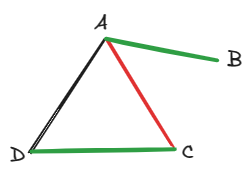
\includegraphics[width=0.25\linewidth]{image.png}
        \caption{A tight example.}
        \label{}
    \end{figure}
    
\end{parts}
\end{Solution}
\newpage

\miquestion
How long does it take you to finish the assignment (including thinking and discussion)?
Give a score (1,2,3,4,5) to the difficulty.
Do you have any collaborators?
Please write down their names here.

\begin{Solution}

These four questions cost 4h, 6h, 2h, 1h respectively (typing also included).

The difficulty scores are 4, 5, 3, 2 respectively.

I complete this assignment independently.
\end{Solution}

\end{questions}
\end{document}
